\section{Ansichten und Funktionen}
Im Folgenden werden die Funktionen der App erläutert. Alle Ansichten sind in Abbildung \ref{fig:overview} dargestellt.

\subsection{Auswahl der Festival-Wochenenden}
Beim Starten der Anwendung erreicht man die Ansicht zur Auswahl eines Festival-Wochenendes. Für jedes Wochenende gibt es eine Seite, zwischen welchen durch das Wischen nach links und rechts gewechselt werden kann. Diese Seiten enthalten ein Bild in der Farbe des jeweiligen Wochenendes, sowie die wichtigsten Informationen. Durch das Auswählen einer dieser Seiten wird man zur Übersicht des Wochenendes weitergeleitet.

\subsection{Hinweis beim ersten Start der Anwendung}
Beim ersten Start der Anwendung wird ein Hinweis angezeigt, mit kurzen Informationen zum Nutzen der App. Durch das Klicken auf einen Button wird gespeichert, dass der Hinweis in Zukunft nicht mehr angezeigt wird.

\subsection{Übersicht eines Festival-Wochenendes}
Die Übersicht eines Festival-Wochenendes besteht aus der Werke Übersicht, sowie aus der Künstler Übersicht. Des Weiteren gibt es ein Menü in der Toolbar, durch welches man auf weitere Ansichten mit zusätzlichen Informationen gelangen kann (vgl. Abschnitt \nameref{sec:navigation}).

\subsection{Werke Übersicht}
Alle Werke des ausgewählten Wochenendes sind in der Werke Übersicht zufällig durchmischt dargestellt (siehe Abbildung \ref{fig:werke}). Bei Klick auf ein Werk öffnet sich die Detailansicht zu diesem Werk.

\begin{figure}[h]
    \centering
        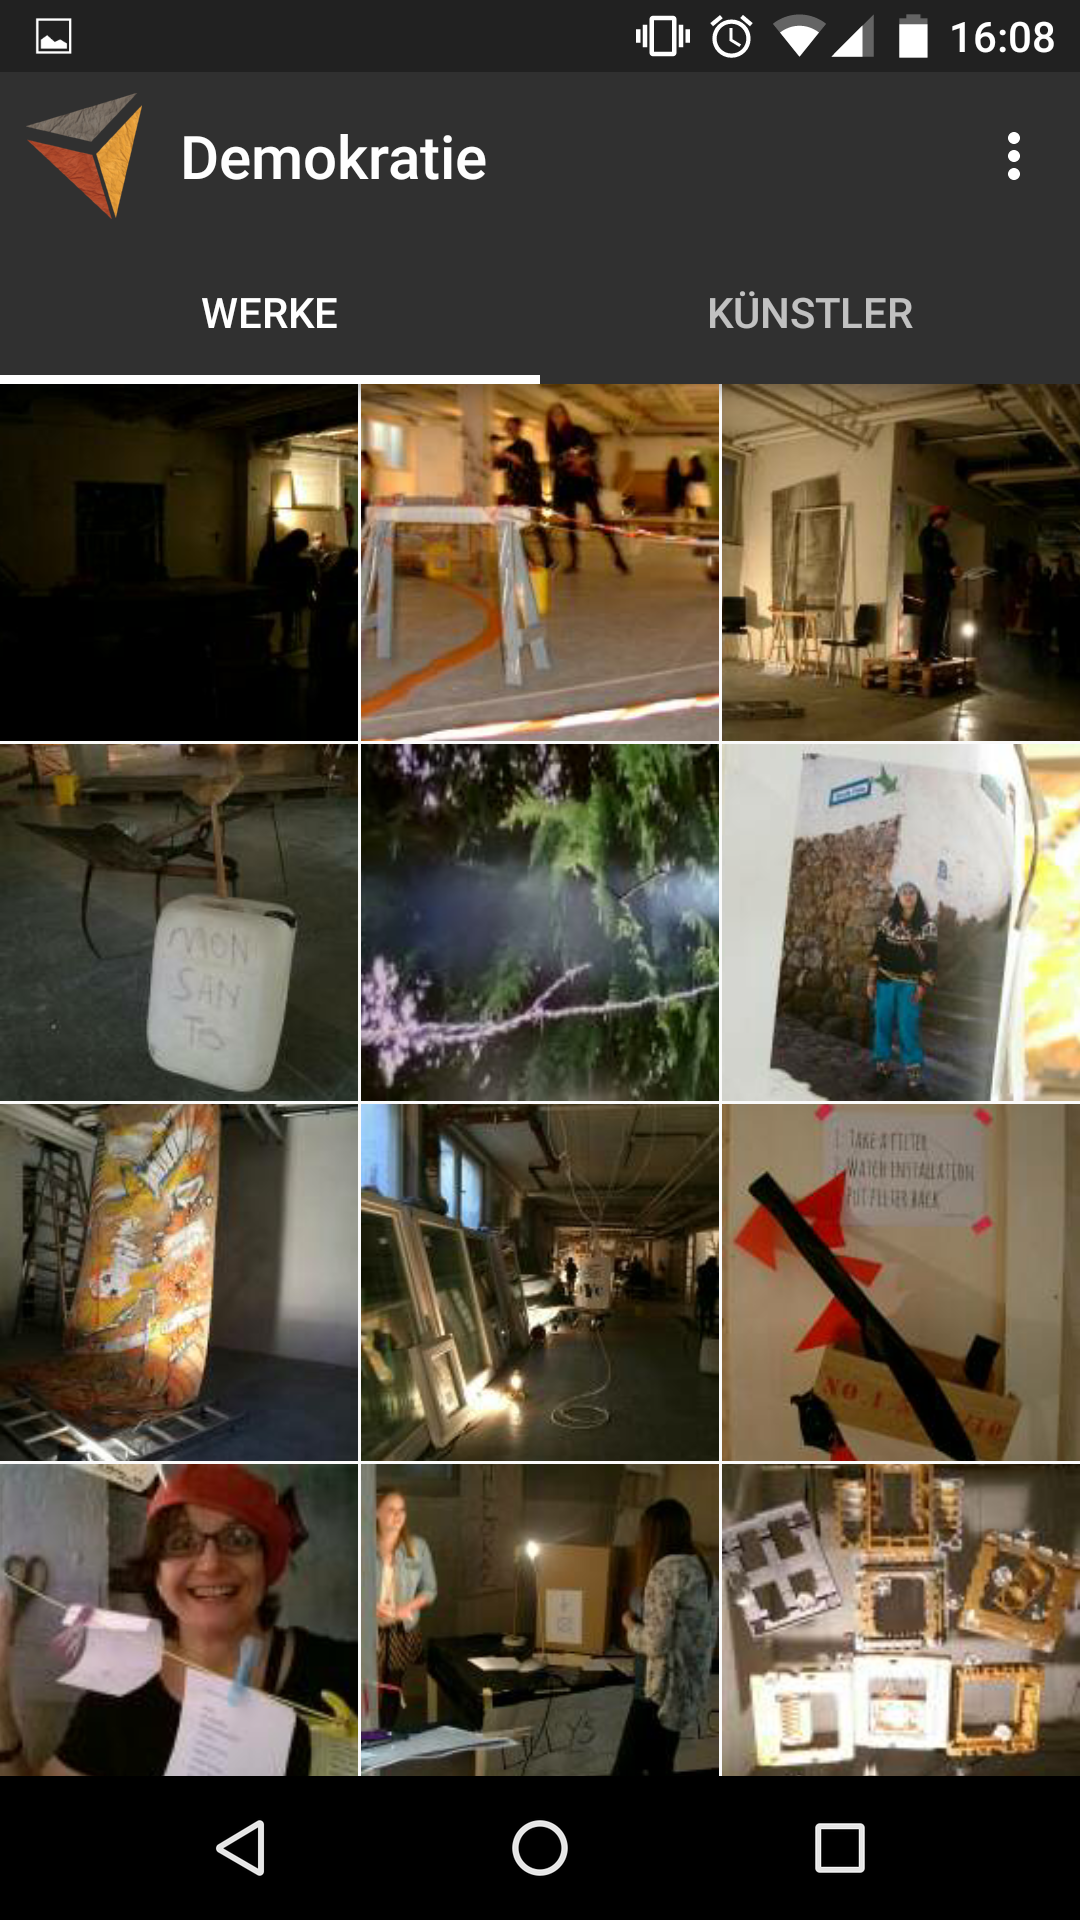
\includegraphics[width=.25\textwidth]{figures/werke.png}
    \caption{Werke Übersicht}
    \label{fig:werke}
\end{figure}

\subsection{Künstler Übersicht}
Die Künstler des Festival-Wochenendes sind in der Übersicht durch ein Profilbild und den Namen handgeschrieben dargestellt. Durch das Auswählen eines Künstlers kann man auf der Künstler Detail Ansicht weitere Werke und mehr Informationen zu diesem Künstler erfahren.

\subsection{Werke Detail Ansicht}
Die Werke Detail Ansicht besteht aus einem Viewpager. Das bedeutet, dass durch das Swipen sofort andere Werke erscheinen. In der Detail Ansicht wird lediglich das Werk auf schwarzem Hintergrund angezeigt, welches durch Zoomen vergrößert werden kann. Durch Klicken auf das Werk erscheinen die Kontrollelemente der Navigation, sowie der zugehörende Künstler. Durch einen Klick auf den Künstlernamen erreicht man die Künstler Detail Ansicht.

\subsection{Künstler Detail Ansicht}
Die Künstler Detail Ansicht beinhaltet einen Text über den Künstler, sowie Bilder von dessen Werken. Ist der Text zu lange, wird nur ein Teil angezeigt, wobei der ganze Text durch das Ausklappen der Karte angezeigt werden kann. Bei der Auswahl eines Werks des Künstlers wird die Werk Detail Ansicht geöffnet, wobei durch das Swipen nur die Werke dieses Künstlers angezeigt werden. In der Toolbar wird - wie in der Künstler Übersicht - das Profilbild des Künstlers, sowie dessen Name angezeigt. 

\subsection{Anfahrt}
In der Anfahrt Ansicht wird eine Google Maps Karte\footnote{\url{https://maps.google.com/}} mit drei Marken an den Orten in München angezeigt. Jeder Marker ist in der jeweiligen Farbe des Wochenendes (vgl. Abschnitt \nameref{sec:visual}). Beim Klick auf einen der Marker erscheint eine Karte mit Informationen über dieses Event (Name, Datum und Ort des ausgewählten Festival Wochenendes). 

\subsection{Event Informationen}
Zu den Event Informationen gehören das Teaser-Video, eine Beschreibung des Festivals, Termine und Orte, sowie die Gründer des Festivals. Diese Informationen sind über die Ansicht der Event Informationen abrufbar. Da diese Daten viel Platz in Anspruch nehmen, wurden die Beschreibung und die Termine des Festivals in aufklappbare Karten integriert. Die Gründer bestehen aus denselben Elementen wie in der Künstler Übersicht. Durch einen Klick auf eines der Elemente kann man in der Künstler Detail Ansicht mehr über diesen Gründer erfahren.

\subsection{Impressum}
Im Impressum sind Informationen über die Herkunft der Informationen, den Aufbau der Anwendung, sowie rechtliche Absicherungen festgehalten.


\subsection{Navigation}
\label{sec:navigation}
Die Navigation durch die Anwendung wird in Abbildung \ref{fig:overview} dargestellt. Das Menü in der Toolbar ist von der Ansicht zur Auswahl eines Festival-Wochenendes, sowie von der Übersicht eines Festival-Wochenendes aus erreichbar. Dadurch hat der Nutzer die Möglichkeit auf die Anfahrtsansicht, die Ansicht der Event Informationen, sowie das Impressum zu gelangen. Hat der Nutzer ein Wochenende ausgewählt, kann er stets durch den Klick auf das App-Icon in der Toolbar oder auf das Menü-Item "`Events"' zurück zur Übersicht der Festival-Wochenenden geleitet werden. 

\begin{figure*}[p]
    \centering
        \includegraphics[width=.85\textwidth]{figures/overview.png}
    \caption{Navigationsfluss aller Ansichten}
    \label{fig:overview}
\end{figure*}